% ====================================================================

% ====================================================================
\documentclass[article,paper=a4paper]{jlreq}

% jpreportパッケージの読み込み
\usepackage{jpreport}

% ページレイアウトの設定
\usepackage{geometry}
\usepackage{enumitem}
\geometry{
    top=25mm,
    bottom=25mm,
    left=25mm,
    right=25mm
}
% TikZライブラリ
\usetikzlibrary{
    patterns,
    calc,
    arrows,
    decorations,
    decorations.markings,
    angles,
    shapes.geometric,
    fit,
    knots
}
% TikZ用のスタイル
\tikzset{
  every path/.style={
    black,
    line width=1pt
  },
  every node/.style={
    transform shape,
    knot crossing,
    inner sep=1.5pt
  }
}
% ハイパーリンクの設定
\usepackage[unicode]{hyperref}
\usepackage{bookmark}
\usepackage[nameinlink]{cleveref}

\hypersetup{
    colorlinks=true,
    linkcolor=black,
    urlcolor=blue,
    citecolor=blue,
    pdftitle=,
    pdfauthor=
}

% 数学演算子の定義


% cleveref用の日本語設定
\crefname{equation}{式}{式}
\Crefname{equation}{式}{式}
\crefname{thm}{定理}{定理}
\crefname{lem}{補題}{補題}
\crefname{cor}{系}{系}
\crefname{ex}{例}{例}
\crefname{def}{定義}{定義}
\crefname{prop}{命題}{命題}
\crefname{prob}{問題}{問題}

% 色彩の定義
\definecolor{yukari}{RGB}{196, 163, 191}

% 文書情報
\title{現象数理1}
\author{akari0koutya}
\date{\today}

\begin{document}

% --- タイトル ------------------------------------------------------
\maketitle
\begin{abstract}
    曲線と曲面の微分幾何は現代微分幾何の根幹をなす重要な研究分野であり、数学研究としてだけでなく関連諸分野とも関わりを持ちながら研究が進められている。本授業では、平面曲線に焦点を当てて、平面曲線の曲がり具合を記述する「\textbf{曲率}」を数学的に定式化し、曲率が満たす性質をいくつか紹介する．また，懸垂線と弾性曲線と呼ばれる古典的な対象を通して、ある種のエネルギーの最小解・極小解を求める\textbf{変分問題}と、その解から定まる幾何的形状について学ぶことを目的とする。
\end{abstract}
\tableofcontents
%% 本文の内容をここに記述
% ====================================================================
\lecture{第 1 回(2026/04/15)}

\section{ガイダンス}

\subsection{成績}

\begin{itemize}
    \item 平常点 : 50点（4点 $\times$ レポート12問 + アンケート 2点）
    \item 期末試験 : 50点（+10点のボーナス問題有）
    \item  $\min\{\text{平常点}+\text{期末試験},100\}$
\end{itemize}

\section{曲線}

原点中心を中心とした半径 $r$ の円を考える。このとき、円の法事の仕方はいくつかの方法がある。
\begin{itemize}
    \item 円の方程式 : $x^2+y^2=r^2$
    \item パラメーター表示 : $\gamma(t)=(r\cos t, r\sin t)$
    \item グラフ表示 : $y=\sqrt{r^2-x^2}$ と $y=-\sqrt{r^2-x^2}$
    \item 微分方程式 : $\frac{d^2y}{dx^2}=-\frac{1}{r^2}y$
\end{itemize}

\begin{prob}
    双曲線 $x^2-y^2=1$ のパラメーター表示を求めよ。
\end{prob}

\begin{proof}
    $$\gamma(t)=(\cosh t, \sinh t)$$
    とすればよい。ここで、
    \[
    \cosh t = \frac{e^t + e^{-t}}{2}, \quad \sinh t = \frac{e^t - e^{-t}}{2}
    \]
    である。
\end{proof}

この授業では、特に、\textbf{パラメータ表示}について学ぶ。つまり、$C^{\infty}$ 級関数
\[\gamma : \R \supseteq I=[a,b] \to \R^2, \quad t \mapsto (x(t), y(t))\]
を考える。

方程式としての表示が便利でなのは、代数的な性質を調べる場合であり、これに関連した分野は代数幾何である。

速度ベクトルと加速度ベクトルは列ベクトル表記する。すなわち、
\[
\frac{d\gamma}{dt} = \begin{pmatrix} \frac{dx}{dt} \\ \frac{dy}{dt} \end{pmatrix}, \quad \frac{d^2\gamma}{dt^2} = \begin{pmatrix} \frac{d^2x}{dt^2} \\ \frac{d^2y}{dt^2} \end{pmatrix}
\]
として表す。

\begin{dfn}
    \quad $\gamma : I = [a,b] \to \R^2$ が\textbf{正則}であるとは、すべての $t \in I$ に対して $\frac{d\gamma}{dt}(t) \neq 0$ であることをいう。
\end{dfn}

\begin{figure}[htbp]
\centering
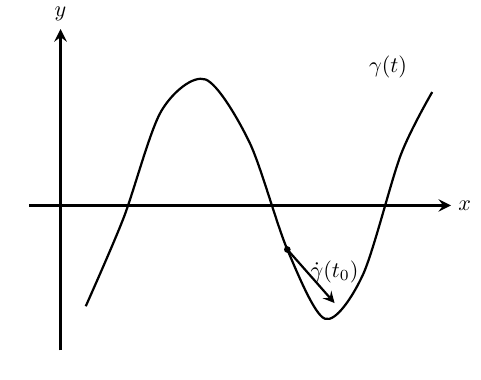
\begin{tikzpicture}[scale=0.8,>=stealth]

    % 座標軸
    \draw[->] (-0.5,0) -- (6.2,0) node[right] {$x$};
    \draw[->] (0,-2.3) -- (0,2.8) node[above] {$y$};

    % 曲線 gamma(t)
    \draw[thick]
        plot[smooth] coordinates {
            (0.4,-1.6)
            (1.0,-0.2)
            (1.6,1.5)
            (2.3,2.0)
            (3.0,1.0)
            (3.6,-0.7)
            (4.2,-1.8)
            (4.8,-1.1)
            (5.4,0.8)
            (5.9,1.8)
        };

    % 曲線のラベル
    \node at (5.2,2.2) {$\gamma(t)$};

    % 点 gamma(t_0)
    \fill (3.6,-0.7) circle (1.5pt);
    \node[below right] at (3.6,-0.7){};

    % 速度ベクトル
    \draw[->,thick] (3.6,-0.7) -- (4.35,-1.55)
        node[above] {$\dot{\gamma}(t_0)$};

\end{tikzpicture}
\caption{正則な曲線の例}
\end{figure}

\begin{ex}
    \quad $\gamma(t) = (r\cos t, r\sin t)$ は $t \in [0, 2\pi]$ で正則である。
    これは、
    \[
    \frac{d\gamma}{dt}(t) = \begin{pmatrix}
-r\sin t \\ r\cos t
    \end{pmatrix}
    \]
    であり、$t \in [0, 2\pi]$ で常にゼロベクトルではないため。
\end{ex}

\begin{ex}
    \quad $\gamma(t) = (t^2, t^3)$ は $t \in \R$ で正則でない。なぜなら、
    \[
    \frac{d\gamma}{dt}(t) = \begin{pmatrix}
2t \\ 3t^2
    \end{pmatrix}
    \]
    であり、$t=0$ のときゼロベクトルになるため。
\end{ex}

\begin{dfn}
    \quad $\gamma(t)$ : $C^{\infty}$ 級関数\\
    速度ベクトル $\frac{d\gamma}{dt}(t)$ の値がゼロベクトルになる点 $t$ を $\gamma$ の\textbf{特異点}という。
\end{dfn}

\begin{ex}
    \quad 上で確認したように、$\gamma(t) = (t^2, t^3)$ は $t=0$ で特異点を持つ。
\end{ex}

\begin{figure}[htbp]
\centering
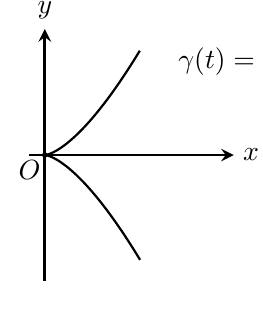
\begin{tikzpicture}[scale=1,>=stealth]
    % 座標軸
    \draw[->] (-0.2,0) -- (2.4,0) node[right] {$x$};
    \draw[->] (0,-1.6) -- (0,1.6) node[above] {$y$};

    % 曲線 gamma(t) = (t^2, t^3)
    \draw[thick,domain=-1.1:1.1,samples=200,smooth,variable=\t]
        plot ({\t*\t},{\t*\t*\t});

    % 原点
    \fill (0,0) circle (1pt);
    \node[below left] at (0,0) {$O$};

    % ラベル
    \node[right] at (1.6,1.2) {$\gamma(t)=(t^2,t^3)$};
\end{tikzpicture}
\caption{曲線 gamma(t)（x座標が t の二乗、y座標が t の三乗）}
\label{fig:gamma-t2-t3}
\end{figure}

\begin{dfn}
    \quad $\gamma(t) \in \R^2 : C^{\infty}$ , $\|\cdot\|$ : Euclid ノルム \\
    このとき、
    \[L \coloneq \int_a^b \left\|\frac{d\gamma}{dt}(t)\right\| \,dt\]     
    を\textbf{曲線} $\gamma$ \textbf{の長さ}という。
\end{dfn}

\begin{prob}
    \quad サイクロイド $\gamma(t) = (t - \sin t, 1 - \cos t)$ を考える。
    \begin{itemize}
        \item $\gamma$ は $\R$ 上正則か？
        \item $\gamma \quad (t \in [0, 2\pi])$ の長さを求めよ。
    \end{itemize}
\end{prob}

\begin{proof}
    一つ目に関して、
    \begin{align*}
        \frac{d\gamma}{dt}(t) &= \begin{pmatrix}
1 - \cos t \\ \sin t
        \end{pmatrix}
    \end{align*}

    である。したがって、$\frac{d\gamma}{dt}(t) = 0$ となるのは $t=0$ と $t=2\pi$ のときである。したがって、$\gamma$ は $\R$ 上正則でない。

    二つ目に関して、
    \begin{align*}
        L &= \int_0^{2\pi} \left\|\frac{d\gamma}{dt}(t)\right\| \,dt \\
        &= \int_0^{2\pi} \sqrt{(1 - \cos t)^2 + (\sin t)^2} \,dt \\
        &= \int_0^{2\pi} \sqrt{2 - 2\cos t} \,dt \\
        &= \int_0^{2\pi} 2\sin\left(\frac{t}{2}\right) \,dt \\
        &= 4 \int_0^{\pi} \sin u \,du \quad (u = t/2) \\
        &= 4 \left[-\cos u\right]_0^{\pi} \\
        &= 4 (1 + 1) \\
        &= 8
    \end{align*}
\end{proof}

\begin{prob}
    \quad $a > 0$ : 定数\\
    曲線
    \[\gamma(t) = \begin{pmatrix}
        \left(1+a\right)\cos t-a\cos\left(\frac{1+a}{a}t\right)\\(1+a)\sin t-a\sin\left(\frac{1+a}{a}t\right)\end{pmatrix},\quad t \in [0, 2\pi a]\]
    の長さを求めよ。この曲線を\textbf{エピサイクロイド}と呼ぶ。
\end{prob}        

\begin{proof}
    \begin{align*}
        \frac{d\gamma}{dt}(t) &= \begin{pmatrix}
        -(1+a)\sin t + (1+a)\sin\left(\frac{1+a}{a}t\right) \\
        (1+a)\cos t - (1+a)\cos\left(\frac{1+a}{a}t\right)
        \end{pmatrix}\\
        &= (1+a) \begin{pmatrix}
        -\sin t + \sin\left(\frac{1+a}{a}t\right) \\
        \cos t - \cos\left(\frac{1+a}{a}t\right)
        \end{pmatrix}
    \end{align*}

    である。したがって、

    \begin{align*}
        L &= \int_0^{2\pi a} \left\|\frac{d\gamma}{dt}(t)\right\| \,dt \\
        &= (1+a) \int_0^{2\pi a} \sqrt{(-\sin t + \sin\left(\frac{1+a}{a}t\right))^2 + (\cos t - \cos\left(\frac{1+a}{a}t\right))^2} \,dt \\
        &= (1+a) \int_0^{2\pi a} \sqrt{2 - 2\cos\left(\frac{1+a}{a}t - t\right)} \,dt \\
        &= (1+a) \int_0^{2\pi a} 2\sin\left(\frac{1}{2}\left(\frac{1+a}{a}t - t\right)\right) \,dt \\
        &= 2(1+a) \int_0^{2\pi a} \sin\left(\frac{t}{2a})\right) \,dt \\
        &= 4a(1+a) \int_0^{\pi} \sin u \,du \quad (u = t/(2a)) \\
        &= 4a(1+a) \left[-\cos u\right]_0^{\pi} \\
        &= 4a(1+a) (1 + 1) \\
        &= 8a(1+a)
    \end{align*}
\end{proof}

\begin{dfn}
    \quad $\gamma(t)$ : $C^{\infty}$ 級関数, 正則\\
    \[S(t) \coloneq \int_a^t \left\|\frac{d\gamma}{du}(u)\right\| \,d u \]
    を曲線 $\gamma$ の \textbf{弧長関数}という。
\end{dfn}

\begin{lem}
    \quad $\gamma(t)$ : $C^{\infty}$ 級関数, 正則\\
    このとき、$S(t)$ は $C^{\infty}$ 級関数であり、$S'(t) = \left\|\frac{d\gamma}{dt}(t)\right\|$ が成り立つ。つまり、$S(t)$ は単調増加関数である。
\end{lem}

\begin{proof}
    微分積分学の基本定理より、
    \[S'(t) = \left\|\frac{d\gamma}{dt}(t)\right\| \geq 0\]
    である。ここで、$\gamma$ の正則性より、$\frac{d\gamma}{dt}(t) \neq 0$ であるため、$S'(t) > 0$ が成り立つ。したがって、$S(t)$ は単調増加関数である。
\end{proof}

\lecture{第2回 : (2026/04/22)}

\begin{thm}[逆関数定理]
    \quad $f : U \to V$ : $C^{1}$ 級関数, $U,V$ : 開集合\\
    このとき、$f$ の微分が全ての点で可逆であるならば、$f$ は局所的に逆関数を持ち、その逆関数も $C^{1}$ 級関数である。
\end{thm}

今、$S(t)$ は単調増加関数であるため、逆関数定理より、$S(t)$ は逆関数 $t(s) = S^{-1}(s)$ を持ち、これは $C^{1}$ 級関数である。よって、
\[\therefore \gamma = \gamma(t) = \gamma(t(s)).\]

以降、$\gamma$ を $s$ の関数とみなして、
\[\gamma(s) = \gamma(t(s)) = \left(x(s),y(s)\right)\]
 と表すことにする。これを\textbf{弧長パラメータ表示}という。ここでは、
 \[\gamma^{\prime} := \frac{d\gamma}{ds} = \begin{pmatrix}
    x^{\prime}(s) \\ y^{\prime}(s)
 \end{pmatrix}\]
 と表すことにする。

\begin{rem}
    $\gamma = \gamma(s)$ とあららされるとき、$\gamma$ は\textbf{弧長パラメータ表示されている}という。
\end{rem}

\begin{prop}
    \quad $\gamma(s)$ : 弧長パラメータ表示\\
    このとき、$\|\gamma^{\prime}(s)\| = 1$ が成り立つ。
\end{prop}

\begin{proof}
    弧長パラメータ表示の定義より、
    \[\|\gamma^{\prime}(s)\| = \left\|\frac{d\gamma}{ds}\right\| = \left\|\frac{d\gamma}{dt}\cdot \frac{dt}{ds}\right\| = \left\|\frac{d\gamma}{dt} \cdot \frac{1}{\frac{dS}{dt}}\right\| = \left\|\frac{d\gamma}{dt} \cdot \frac{1}{\left\|\frac{d\gamma}{dt}\right\|} \right\| = 1\]
    が成り立つ。
\end{proof}

以降、$\gamma$ を弧長パラメータ表示されているとみなして、$\gamma(s)$ と表すことにする。

\begin{dfn}
    \quad $\gamma(s)$ : 弧長パラメータ表示\\
    このとき、
    \[n(s) := \begin{pmatrix}
        0 & -1\\
        1 & 0
    \end{pmatrix}\gamma^{\prime}(s)\]
    を曲線 $\gamma$ の\textbf{単位法線ベクトル}(unit normal vector)という。また、組 $(\gamma^{\prime}(s), n(s))$ を曲線 $\gamma$ の\textbf{動標高}という。
\end{dfn}

\begin{rem}
    単位法線ベクトル $n(s)$ は、$\gamma^{\prime}(s)$ を $90$ 度回転させたベクトルである。すなわち、回転行列 $\begin{pmatrix}
        \sin\theta & -\cos\theta\\
        \cos\theta & \sin\theta
    \end{pmatrix}$ に $\theta = \FRAC{\pi}{2}$ を代入した行列を $\gamma^{\prime}(s)$ に作用させることで得られる。
\end{rem}

\begin{rem}
    動標高 $(\gamma^{\prime}(s), n(s))$ は $\R^2$ の正規直交基底をなす。すなわち、$\gamma^{\prime}(s)$ と $n(s)$ は互いに直交し、両方とも単位ベクトルである。
\end{rem}

    さて、$\left\|\gamma^{\prime}(s)\right\| = 1$ であるから、
    \[\left\|\gamma^{\prime}\right\|^2 = \gamma^{\prime} \cdot \gamma^{\prime} = 1\]
    である。これを、$\gamma^{\prime} \cdot \gamma^{\prime} = 1$ の両辺を $s$ で微分すると、
    \[2\gamma^{\prime} \cdot \gamma^{\prime\prime} = 0\]
    なので、$\gamma^{\prime} \cdot \gamma^{\prime\prime} = 0$ が成り立つ。
    よって、速度ベクトル $\gamma^{\prime}(s)$ と加速度ベクトル $\gamma^{\prime\prime}(s)$ は直交する。すなわち、$\gamma^{\prime\prime}(s)$ は単位法線ベクトル $n(s)$ と平行である。したがって、ある関数 $\kappa(s)$ が存在して、
\begin{equation}
        \gamma^{\prime\prime}(s) = \kappa(s) n(s)
        \label{eq:gamma-pp}
    \end{equation}
    が成り立つ。

\begin{prob}
    \cref{eq:gamma-pp} が成り立つことを示せ。
\end{prob}

\begin{proof}
    $(\gamma^{\prime}(s), n(s))$ は $\R^2$ の正規直交基底であるから、任意のベクトルは
    \[
        \bigl(v \cdot \gamma^{\prime}(s)\bigr)\gamma^{\prime}(s) + \bigl(v \cdot n(s)\bigr)n(s)
    \]
    と一意的に表される。これを $v = \gamma^{\prime\prime}(s)$ に適用すると、
    \[
        \gamma^{\prime\prime}(s)
        = \bigl(\gamma^{\prime\prime}(s) \cdot \gamma^{\prime}(s)\bigr)\gamma^{\prime}(s)
        + \bigl(\gamma^{\prime\prime}(s) \cdot n(s)\bigr)n(s)
    \]
    を得る。ところが、すでに $\gamma^{\prime}(s) \cdot \gamma^{\prime\prime}(s) = 0$ を示したので、
    \[
        \gamma^{\prime\prime}(s) = \bigl(\gamma^{\prime\prime}(s) \cdot n(s)\bigr)n(s)
    \]
    となる。したがって、$\kappa(s) := \gamma^{\prime\prime}(s) \cdot n(s)$ とおけば \cref{eq:gamma-pp} が成り立つ。
\end{proof}

\begin{dfn}
    上で定義した関数 $\kappa(s)$ を曲線 $\gamma$ の\textbf{曲率}という。
\end{dfn}

\begin{prop}
    先の議論より、
    \[\kappa(s) = \gamma^{\prime\prime} \cdot n(s) = \det(\gamma^{\prime}, \gamma^{\prime\prime}) .\]
    また、$\gamma^{\prime\prime} = 0$ のとき、$\kappa(s) = 0$ である。
\end{prop}

\begin{proof}
    すでに
    \[
        \gamma^{\prime\prime}(s) = \kappa(s)n(s)
    \]
    が成り立ち、$n(s)$ は単位ベクトルであるから、
    \[
        \gamma^{\prime\prime}(s) \cdot n(s) = \kappa(s) n(s) \cdot n(s) = \kappa(s)
    \]
    を得る。
    また、
    \[
        n(s) =
        \begin{pmatrix}
            0 & -1\\
            1 & 0
        \end{pmatrix}\gamma^{\prime}(s)
    \]
    である。ここで、$\gamma^{\prime}(s) = \begin{pmatrix}x^{\prime}(s)\\ y^{\prime}(s)\end{pmatrix}$,
    $\gamma^{\prime\prime}(s) = \begin{pmatrix}x^{\prime\prime}(s)\\ y^{\prime\prime}(s)\end{pmatrix}$ と書くと、
    \begin{align*}
        \gamma^{\prime\prime}(s) \cdot n(s)
        &= \begin{pmatrix}
        x^{\prime\prime}(s)\\
        y^{\prime\prime}(s)
        \end{pmatrix}
        \cdot
        \left(
        \begin{pmatrix}
        0 & -1\\
        1 & 0
        \end{pmatrix}
        \begin{pmatrix}
        x^{\prime}(s)\\
        y^{\prime}(s)
        \end{pmatrix}
        \right) \\
        &= \begin{pmatrix}
        x^{\prime\prime}(s)\\
        y^{\prime\prime}(s)
        \end{pmatrix}
        \cdot
        \begin{pmatrix}
        -y^{\prime}(s)\\
        x^{\prime}(s)
        \end{pmatrix} \\
        &= x^{\prime\prime}(s)(-y^{\prime}(s)) + y^{\prime\prime}(s)x^{\prime}(s) \\
        &= x^{\prime}(s)y^{\prime\prime}(s) - y^{\prime}(s)x^{\prime\prime}(s) \\
        &= \det\begin{pmatrix}
        x^{\prime}(s) & x^{\prime\prime}(s)\\
        y^{\prime}(s) & y^{\prime\prime}(s)
        \end{pmatrix} \\
        &= \det(\gamma^{\prime}(s), \gamma^{\prime\prime}(s)).
    \end{align*}
    したがって、
    \[
        \kappa(s) = \gamma^{\prime\prime}(s) \cdot n(s) = \det(\gamma^{\prime}(s), \gamma^{\prime\prime}(s))
    \]
    である。さらに、$\gamma^{\prime\prime}(s) = 0$ ならば
    \[
        \kappa(s) = \gamma^{\prime\prime}(s) \cdot n(s) = 0
    \]
    となる。
\end{proof}

\begin{ex}
    \quad $\gamma(s) = (R\cos s, R\sin s) \, (s \in [0, 2\pi]\, R > 0)$\\
    このときの曲率 $\kappa(s)$ を求める。
    $\gamma^{\prime} = \begin{pmatrix}
        -R\sin s \\ 
        R\cos s
    \end{pmatrix}$ なので、
    \[S = \int_{0}^{s}\left\|\begin{pmatrix}
        -R\sin t\\
        R\cos t
    \end{pmatrix}\right\|\,dt = \int_{0}^{s} R \, dt = Rs.\]
    したがって、
    \begin{align*}
        \gamma(s) &= \left(R\cos\frac{S}{R}, R\sin\frac{S}{R}\right)\\
        \gamma^{\prime}(s) &= \begin{pmatrix}
        -\sin\frac{S}{R} \\
        \cos\frac{S}{R}
        \end{pmatrix}\\
        \gamma^{\prime\prime}(s) &= \begin{pmatrix}
        -\frac{1}{R}\cos\frac{S}{R} \\
        -\frac{1}{R}\sin\frac{S}{R}
        \end{pmatrix}\\
        \kappa(s) &= \det(\gamma^{\prime}, \gamma^{\prime\prime}) \\
        &= \det\left(\begin{pmatrix}
        -\sin\frac{S}{R} &  -\frac{1}{R}\cos\frac{S}{R}\\
        \cos\frac{S}{R} & -\frac{1}{R}\sin\frac{S}{R}
        \end{pmatrix}\right) \\
        &= \frac{1}{R}
    \end{align*}
\end{ex}

\begin{prob}
    \[\gamma(s) = (R\cos s, -R\sin s) \, (s \in [0, 2\pi]\, R > 0)\]
    この曲率 $\kappa(s)$ を求めよ。
\end{prob}

\begin{proof}
    $\gamma^{\prime} = \begin{pmatrix}
        -R\sin s \\ 
        -R\cos s
    \end{pmatrix}$ なので、
    \[S = \int_{0}^{s}\left\|\begin{pmatrix}
        -R\sin t\\
        -R\cos t
    \end{pmatrix}\right\|\,dt = \int_{0}^{s} R \, dt = Rs.\]
    したがって、
    \begin{align*}
        \gamma(s) &= \left(R\cos\frac{S}{R}, -R\sin\frac{S}{R}\right)\\
        \gamma^{\prime}(s) &= \begin{pmatrix}
        -\sin\frac{S}{R} \\
        -\cos\frac{S}{R}
        \end{pmatrix}\\
        \gamma^{\prime\prime}(s) &= \begin{pmatrix}
        -\frac{1}{R}\cos\frac{S}{R} \\
        \frac{1}{R}\sin\frac{S}{R}
        \end{pmatrix}\\
        \kappa(s) &= \det(\gamma^{\prime}, \gamma^{\prime\prime}) \\
        &= \det\left(\begin{pmatrix}
        -\sin\frac{S}{R} &  -\frac{1}{R}\cos\frac{S}{R}\\
        -\cos\frac{S}{R} & \frac{1}{R}\sin\frac{S}{R}
        \end{pmatrix}\right) \\
        &= -\frac{1}{R}
    \end{align*}
    
\end{proof}

\begin{figure}[htbp]
\centering
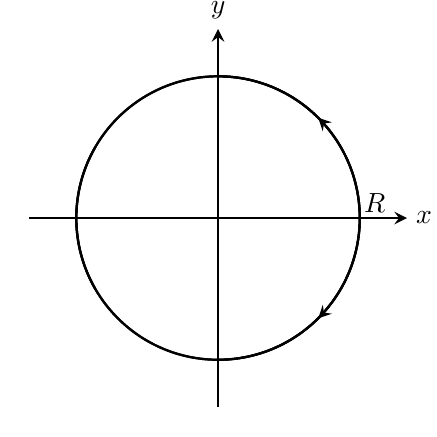
\begin{tikzpicture}[scale=1,>=stealth]
    % 座標軸
    \draw[->] (-2.4,0) -- (2.4,0) node[right] {$x$};
    \draw[->] (0,-2.4) -- (0,2.4) node[above] {$y$};

    % 円（半径 R）
    \draw[thick] (0,0) circle (1.8);
    \draw[thick] (0,0) -- (1.8,0) node[above right] {$R$};

    % 時計回りの矢印
    \draw[thick,postaction={decorate},
        decoration={markings, mark=at position 0.45 with {\arrow{stealth}}}]
        (0,1.8) arc (90:-210:1.8);

    % 反時計回りの矢印
    \draw[thick,postaction={decorate},
        decoration={markings, mark=at position 0.45 with {\arrow{stealth}}}]
        (0,-1.8) arc (-90:210:1.8);
\end{tikzpicture}
\caption{$x$ 軸・$y$ 軸上の半径 $R$ の円と回転方向}
\end{figure}

\lecture{第3回 : (2026/04/30)}

\section{曲率の不変性(その1)}

幾何学とは何か？幾何学とは、空間の不変量を研究する学問である。例えば、点と線の距離、曲線の長さ、曲面の面積などが普遍量である。これらの普遍量は、空間の構造に依存しないため、幾何学的な性質を表すことができる。

\begin{ex}
    二つの曲線を回転させて移動させて重なるとき、対応する各点の曲率は等しいはずである。
\end{ex}

\begin{thm}
    \quad $\gamma(s)$ : 弧長パラメータ表示された曲線\\
    $\gamma$ の曲率 $\kappa(s)$ は、回転と並行移動で不変である。すなわち、
    \[A\in \SO(2) := \{R \in \SL(2,\R) \mid {}^\top R\cdot R = \id, \det R = 1\}, \quad \bm{b} \in \R^2\]
    に対し、曲線
\[\tilde{\gamma}(s) := A\gamma(s) + \bm{b}\]
の曲率 $\tilde{\kappa}(s)$ は $\kappa(s)$ と等しい。
\end{thm}

\begin{rem}
    $ A \in \SO(2)$ は回転を表し、$\bm{b} \in \R^2$ は並行移動を表す。したがって、$\tilde{\gamma}(s)$ は $\gamma(s)$ を回転させてから並行移動させた曲線である。
\end{rem}

\begin{proof}
    今、$\tilde{\gamma}(s) = A\gamma(s) + \bm{b}$ と定義されているから、
    \begin{align*}
    \norm{\tilde{\gamma}^{\prime}(s)} &= \gamma^{\prime}(s)\cdot \gamma^{\prime}(s) \\
    &= {}^\top(\tilde{\gamma}^{\prime}(s)) \cdot \tilde{\gamma}^{\prime}(s) \\
    &= {}^\top(A\gamma^{\prime}(s)) \cdot A\gamma^{\prime}(s) \\
    &= {}^\top \gamma^{\prime}(s) \cdot {}^\top A \cdot A \cdot \gamma^{\prime}(s) \\
    &= {}^\top \gamma^{\prime}(s) \cdot \gamma^{\prime}(s) \\
    &= 1
    \end{align*}
    であり、
    \begin{align*}
        \tilde{\kappa}(s) &= \det(\tilde{\gamma}^{\prime}(s), \tilde{\gamma}^{\prime\prime}(s)) \\
        &= \det(A\gamma^{\prime}(s), A\gamma^{\prime\prime}(s)) \\
        &= \det A \cdot \det(\gamma^{\prime}(s), \gamma^{\prime\prime}(s)) \\
        &= 1 \cdot \kappa(s) \\
        &= \kappa(s)
    \end{align*}
    である。したがって、$\tilde{\kappa}(s) = \kappa(s)$ である。
\end{proof}

\begin{prop}
    $\SO(2) = \left\{R_\theta = \begin{pmatrix}
        \cos\theta & -\sin\theta\\
        \sin\theta & \cos\theta
    \end{pmatrix} \relmid | \theta \in \R\right\}$ である。したがって、回転は角度 $\theta$ によって完全に決まる。
\end{prop}

\begin{proof}[$\supseteq $ の証明]
    $R \in \left\{R_\theta = \begin{pmatrix}
        \cos\theta & -\sin\theta\\
        \sin\theta & \cos\theta
    \end{pmatrix} \relmid | \theta \in \R\right\}$ とすると、
    \[\det R = \begin{pmatrix}
        \cos\theta & -\sin\theta\\
        \sin\theta & \cos\theta
    \end{pmatrix} = 1\] であり、また、
    \[{}^\top R \cdot R = \begin{pmatrix}
        \cos\theta & \sin\theta\\
        -\sin\theta & \cos\theta
    \end{pmatrix} \cdot \begin{pmatrix}
        \cos\theta & -\sin\theta\\
        \sin\theta & \cos\theta
    \end{pmatrix} = \id\] である。したがって、$R \in \SO(2)$ である。
\end{proof}

\begin{proof}[$\subseteq$ の証明]
    $R \in \SO(2)$ とする。$R = (\bm{e}_1, \bm{e}_2)$ とおくと、${}^\top R = \begin{pmatrix}
        {}^\top \bm{e}_1\\
        {}^\top \bm{e}_2
    \end{pmatrix}$ であるから、
    \begin{align*}
        {}^\top R \cdot R &= \begin{pmatrix}
        {}^\top \bm{e}_1\\
        {}^\top \bm{e}_2
    \end{pmatrix} \cdot (\bm{e}_1, \bm{e}_2) \\
    &= \begin{pmatrix}
        {}^\top \bm{e}_1 \cdot \bm{e}_1 & {}^\top \bm{e}_1 \cdot \bm{e}_2\\
        {}^\top \bm{e}_2 \cdot \bm{e}_1 & {}^\top \bm{e}_2 \cdot \bm{e}_2
    \end{pmatrix}\\
    &= \begin{pmatrix}
        \bm{e}_1\bm{e}_1 & \bm{e}_1\bm{e}_2\\
        \bm{e}_2\bm{e}_1 & \bm{e}_2\bm{e}_2
    \end{pmatrix} \\
    &= \begin{pmatrix}
        1 & 0\\
        0 & 1
    \end{pmatrix} = \id
    \end{align*}
    よって、$\bm{e}_1 \cdot \bm{e}_2 = 0$ 、つまり $\bm{e}_1$ と $\bm{e}_2$ は直交する。また、$\norm{\bm{e}_1} = 1$ より、$\bm{e}_1 = \begin{pmatrix} \cos\theta \\ \sin\theta \end{pmatrix}$ と表すことができる。先ほど示したように、$\bm{e}_2$ は $\bm{e}_1$ と直交する単位ベクトルであるから、$\bm{e}_2 = \begin{pmatrix} -\sin\theta \\ \cos\theta \end{pmatrix}$ と表すことができる。したがって、
\[R = (\bm{e}_1, \bm{e}_2) = \begin{pmatrix}
        \cos\theta & -\sin\theta\\
        \sin\theta & \cos\theta
    \end{pmatrix} = R_\theta\]
である。したがって、$R \in \left\{R_\theta = \begin{pmatrix}
        \cos\theta & -\sin\theta\\
        \sin\theta & \cos\theta
    \end{pmatrix} \relmid | \theta \in \R\right\}$ である。
    
\end{proof}

\begin{prob}
    以下を示せ : 
    \begin{enumerate}[label=(\arabic*)\,]
        \item $\SO(2)$ は通常の行列の積に関してアーベル群になることを示せ。
        \item $\operatorname{O}(2)$ がアーベル群でないことを示せ。
    \end{enumerate}
\end{prob}

\begin{proof}[(1) の証明]
    $R_\theta, R_\phi \in \SO(2)$ とする。すると、
    \[
        R_\theta R_\phi = R_{\theta + \phi}
    \]
    である。したがって、$\SO(2)$ は行列の積に関して閉じている。また、$R_0 = \id$ であるから、単位元が存在する。さらに、$R_{-\theta} = R_\theta^{-1}$ であるから、逆元が存在する。最後に、$R_\theta R_\phi = R_{\theta + \phi} = R_{\phi + \theta} = R_\phi R_\theta$ であるから、$\SO(2)$ はアーベル群である。
\end{proof}

\begin{proof}[(2) の証明]
    例えば、$R = \begin{pmatrix}
        1 & 0\\
        0 & -1
    \end{pmatrix}$ と $S = \begin{pmatrix}
        0 & 1\\
        1 & 0
    \end{pmatrix}$ を考えると、確かにこれらは
    \begin{align*}
        {}^\top R \cdot R &= \begin{pmatrix}
            1 & 0\\
            0 & -1
        \end{pmatrix} \cdot \begin{pmatrix}
            1 & 0\\
            0 & -1
    \end{pmatrix} &= \id\\
        {}^\top S \cdot S &= \begin{pmatrix}
            0 & 1\\
            1 & 0
        \end{pmatrix} \cdot \begin{pmatrix}
            0 & 1\\
            1 & 0
    \end{pmatrix} &= \id
    \end{align*}
    であるから、$R, S \in \operatorname{O}(2)$ である。しかし、
    \[
        RS = \begin{pmatrix}
        0 & 1\\
        -1 & 0
    \end{pmatrix} \neq \begin{pmatrix}
        0 & -1\\
        1 & 0
    \end{pmatrix} = SR
    \]
    である。したがって、$\operatorname{O}(2)$ はアーベル群でない。
\end{proof}

\lecture{第4回 : (2026/05/13)}

\section{一般の曲線の曲率}
    一般に、弧長パラメーター表示を求めるのは困難である。そこで、弧長パラメーター表示を求めなくても曲率を定義できるようにすることが望ましい。以下では、一般の曲線の曲率を定義する方法を説明する。

\begin{prob}
    \quad $\gamma(t) = \left(t, \frac{1}{2}t^2\right)$ : 曲線.\\
    このとき、以下を求めよ :
    \[S(t) = \int_0^t\left\lVert \dot{\gamma}(u)\right\rVert \, du \]
\end{prob}

\begin{thm}
    \quad $\gamma(t)=(x(t), y(t))$ : 曲線\\
    このとき、$\gamma$ の曲率 $\kappa(t)$ は、
\[\kappa(t) := \frac{\det(\dot{\gamma}(t), \ddot{\gamma}(t))}{\left\|\dot{\gamma}(t)\right\|^3} = \frac{\dot{x}(t)\ddot{y}(t) - \dot{y}(t)\ddot{x}(t)}{\left((\dot{x}(t))^2 + (\dot{y}(t))^2\right)^{\FRAC{3}{2}}}\]
で定義される。\\
    特に、$y = f(x)$ という形で表される曲線の曲率は、
    \[\kappa(x) = \frac{\ddot{y}}{(1 + (\dot{y})^2)^{\FRAC{3}{2}}}, \quad \left(\dot{y} = \frac{dy}{dx}\, \ddot{y} = \frac{d^2y}{dx^2}\right)\]
    で与えられる。
\end{thm}

\begin{proof}
    まず、
    \begin{align*}
        \gamma^{\prime}(t) &= \frac{d\gamma}{ds}(s) \\
        &= \frac{d\gamma}{dt}\cdot \frac{dt}{ds} \\
        &= \frac{1}{\left\|\dot{\gamma}(t)\right\|}\dot{\gamma}(t)
    \end{align*}
    である。
    次に、
    \begin{align*}
        \gamma^{\prime\prime}(t) &= \frac{d}{ds}\left(\frac{1}{\left\|\dot{\gamma}(t)\right\|}\dot{\gamma}(t)\right) \\
        &= \frac{d}{dt}\left(\frac{1}{\left\|\dot{\gamma}(t)\right\|}\dot{\gamma}(t)\right) \cdot \frac{dt}{ds} \\
        &= \frac{1}{\left\|\dot{\gamma}(t)\right\|}\frac{d}{dt}\left(\frac{1}{\left\|\dot{\gamma}(t)\right\|}\dot{\gamma}(t)\right) \\
        &= \frac{1}{\left\|\dot{\gamma}(t)\right\|}\left(-\frac{1}{\left\|\dot{\gamma}(t)\right\|^2}\left(\dot{\gamma}(t) \cdot \ddot{\gamma}(t)\right)\dot{\gamma}(t) + \frac{1}{\left\|\dot{\gamma}(t)\right\|}\ddot{\gamma}(t)\right) \\
        &= \frac{1}{\left\|\dot{\gamma}(t)\right\|^3}\left(\left\|\dot{\gamma}(t)\right\|^2 \ddot{\gamma}(t) - \left(\dot{\gamma}(t) \cdot \ddot{\gamma}(t)\right)\dot{\gamma}(t)\right)
    \end{align*}
    である。したがって、
    \begin{align*}
        \kappa(t) &= \det(\gamma^{\prime}(t), \gamma^{\prime\prime}(t)) \\
        &= \det\left(\frac{1}{\left\|\dot{\gamma}(t)\right\|}\dot{\gamma}(t), \frac{1}{\left\|\dot{\gamma}(t)\right\|^3}\left(\left\|\dot{\gamma}(t)\right\|^2 \ddot{\gamma}(t) - \left(\dot{\gamma}(t) \cdot \ddot{\gamma}(t)\right)\dot{\gamma}(t)\right)\right) \\
        &= \frac{1}{\left\|\dot{\gamma}(t)\right\|^4}\det\left(\dot{\gamma}(t), \left\|\dot{\gamma}(t)\right\|^2 \ddot{\gamma}(t) - \left(\dot{\gamma}(t) \cdot \ddot{\gamma}(t)\right)\dot{\gamma}(t)\right) \\
        &= \frac{1}{\left\|\dot{\gamma}(t)\right\|^4}\left(\left\|\dot{\gamma}(t)\right\|^2 \det(\dot{\gamma}(t), \ddot{\gamma}(t)) - \left(\dot{\gamma}(t) \cdot \ddot{\gamma}(t)\right)\det(\dot{\gamma}(t), \dot{\gamma}(t))\right) \\
        &= \frac{1}{\left\|\dot{\gamma}(t)\right\|^4}\left(\left\|\dot{\gamma}(t)\right\|^2 \det(\dot{\gamma}(t), \ddot{\gamma}(t))\right) \\
        &= \frac{\det(\dot{\gamma}(t), \ddot{\gamma}(t))}{\left\|\dot{\gamma}(t)\right\|^3}
    \end{align*}
    である。
    特に、$y = f(x)$ という形で表される曲線のとき、$\gamma(t) = (t, f(t))$ と表すことができるから、
    \begin{align*}
        \dot{\gamma}(t) &= (1, \dot{f}(t))\\
        \ddot{\gamma}(t) &= (0, \ddot{f}(t))
    \end{align*}    
    である。したがって、
    \begin{align*}
        \kappa(t) &= \frac{\det(\dot{\gamma}(t), \ddot{\gamma}(t))}{\left\|\dot{\gamma}(t)\right\|^3} \\
        &= \frac{\det\left(\begin{pmatrix}
        1 & 0\\
        \dot{f}(t) & \ddot{f}(t)
        \end{pmatrix}\right)}{\left\|\begin{pmatrix}    1 \\ \dot{f}(t)\end{pmatrix}\right\|^3} \\
        &= \frac{\ddot{f}(t)}{(1 + (\dot{f}(t))^2)^{\FRAC{3}{2}}}
    \end{align*}
    である。
\end{proof}

\begin{prob}
    次の曲線の曲率を求めよ :
    \begin{enumerate}[label=(\arabic*)\,]
        \item 曲線 $\gamma(t) = (a\cos t, b\sin t) \quad (a > 0, b > 0)$ の曲率 $\kappa(t)$ を求めよ。
        \item 極座標表示された曲線 $r = 1 + \cos \theta$ の曲率 $\kappa(\theta)$ を求めよ。
    \end{enumerate}
\end{prob}

\begin{proof}[解答(1)]
    曲率の公式
    \[
        \kappa(t)
        =
        \frac{\dot{x}(t)\ddot{y}(t)-\dot{y}(t)\ddot{x}(t)}
        {\left((\dot{x}(t))^2+(\dot{y}(t))^2\right)^{\FRAC{3}{2}}}
    \]
    を用いる。いま、
    \[
        x(t)=a\cos t,\qquad y(t)=b\sin t
    \]
    であるから、
    \[
        \dot{x}(t)=-a\sin t,\qquad
        \dot{y}(t)=b\cos t
    \]
    であり、さらに
    \[
        \ddot{x}(t)=-a\cos t,\qquad
        \ddot{y}(t)=-b\sin t
    \]
    である。したがって、分子は
    \begin{align*}
        \dot{x}(t)\ddot{y}(t)-\dot{y}(t)\ddot{x}(t)
        &=
        (-a\sin t)(-b\sin t)
        -
        (b\cos t)(-a\cos t)\\
        &=
        ab\sin^2 t+ab\cos^2 t\\
        &=
        ab
    \end{align*}
    となる。また、分母に現れる速度の大きさは
    \[
        \left\|\dot{\gamma}(t)\right\|
        =
        \sqrt{a^2\sin^2 t+b^2\cos^2 t}
    \]
    である。よって、
    \[
        \boxed{
        \kappa(t)
        =
        \frac{ab}
        {\left(a^2\sin^2 t+b^2\cos^2 t\right)^{\FRAC{3}{2}}}
        }
    \]
    である。
\end{proof}  
    
\begin{proof}[解答(2)]
    極座標表示 $r=r(\theta)$ の曲線は
    \[
        \gamma(\theta)
        =
        \left(r(\theta)\cos\theta,\ r(\theta)\sin\theta\right)
    \]
    とパラメーター表示できる。ここで $r'=dr/d\theta$ と書くと、
    \begin{align*}
        \dot{x} &= r'\cos\theta-r\sin\theta,\\
        \dot{y} &= r'\sin\theta+r\cos\theta
    \end{align*}
    であるから、
    \[
        (\dot{x})^2+(\dot{y})^2
        =
        (r')^2+r^2
    \]
    となる。また、
    \begin{align*}
        \ddot{x}
        &=
        r''\cos\theta-2r'\sin\theta-r\cos\theta,\\
        \ddot{y}
        &=
        r''\sin\theta+2r'\cos\theta-r\sin\theta
    \end{align*}
    である。したがって、
    \begin{align*}
        \det(\dot{\gamma},\ddot{\gamma})
        &=
        \dot{x}\ddot{y}-\dot{y}\ddot{x}\\
        &=
        r^2+2(r')^2-rr''
    \end{align*}
    となる。ゆえに、極座標表示された曲線の曲率は
    \[
        \kappa(\theta)
        =
        \frac{r^2+2(r')^2-rr''}
        {\left(r^2+(r')^2\right)^{\FRAC{3}{2}}}
    \]
    で与えられる。

    今回は
    \[
        r=1+\cos\theta
    \]
    であるから、
    \[
        r'=-\sin\theta,\qquad r''=-\cos\theta
    \]
    である。よって、分子は
    \begin{align*}
        r^2+2(r')^2-rr''
        &=
        (1+\cos\theta)^2
        +2\sin^2\theta
        -(1+\cos\theta)(-\cos\theta)\\
        &=
        1+2\cos\theta+\cos^2\theta
        +2(1-\cos^2\theta)
        +\cos\theta+\cos^2\theta\\
        &=
        3+3\cos\theta\\
        &=
        3(1+\cos\theta)
    \end{align*}
    となる。また、
    \begin{align*}
        r^2+(r')^2
        &=
        (1+\cos\theta)^2+\sin^2\theta\\
        &=
        1+2\cos\theta+\cos^2\theta+\sin^2\theta\\
        &=
        2(1+\cos\theta)
    \end{align*}
    である。したがって、$\theta \not\equiv \pi \pmod{2\pi}$ において
    \[
        \kappa(\theta)
        =
        \frac{3(1+\cos\theta)}
        {\left(2(1+\cos\theta)\right)^{\FRAC{3}{2}}}
        =
        \boxed{
        \frac{3}{2^{\FRAC{3}{2}}\sqrt{1+\cos\theta}}
        }.
    \]
    なお、$\theta \equiv \pi \pmod{2\pi}$ では $r=0$ かつ $\dot{\gamma}(\theta)=0$ となるため、通常の曲率公式は適用できない。
\end{proof}

\begin{prob}
    極座標表示された曲線
    \[ r = ae^{b\theta} \quad (a > 0, b > 0, a \neq b) \]
    の曲率 $\kappa(\theta)$ を求めよ。
\end{prob}

\begin{proof}[解答]
    前問と同様に、極座標表示 $r=r(\theta)$ の曲線の曲率公式
    \[
        \kappa(\theta)
        =
        \frac{r^2+2(r')^2-rr''}
        {\left(r^2+(r')^2\right)^{\FRAC{3}{2}}}
    \]
    を用いる。いま、
    \[
        r=ae^{b\theta}
    \]
    であるから、
    \[
        r'=abe^{b\theta}=br,\qquad
        r''=ab^2e^{b\theta}=b^2r
    \]
    である。したがって、分子は
    \begin{align*}
        r^2+2(r')^2-rr''
        &=
        r^2+2b^2r^2-b^2r^2\\
        &=
        (1+b^2)r^2
    \end{align*}
    となる。また、分母は
    \begin{align*}
        \left(r^2+(r')^2\right)^{\FRAC{3}{2}}
        &=
        \left(r^2+b^2r^2\right)^{\FRAC{3}{2}}\\
        &=
        \left((1+b^2)r^2\right)^{\FRAC{3}{2}}\\
        &=
        (1+b^2)^{\FRAC{3}{2}}r^3
    \end{align*}
    である。ここで $a>0$ かつ $e^{b\theta}>0$ より $r>0$ であることを用いた。

    よって、
    \begin{align*}
        \kappa(\theta)
        &=
        \frac{(1+b^2)r^2}{(1+b^2)^{\FRAC{3}{2}}r^3}\\
        &=
        \frac{1}{\sqrt{1+b^2}\,r}\\
        &=
        \boxed{
        \frac{e^{-b\theta}}{a\sqrt{1+b^2}}
        }.
    \end{align*}
\end{proof}

\section{曲率の不変性(その2)}

\begin{thm}
    \quad $\gamma(t)$ : 曲線, $t = t(\tilde{t})$, $\frac{dt}{d\tilde{t}} > 0$, $\kappa(t)$ : $\gamma$ の曲率, $\tilde{\kappa}(\tilde{t})$ : $\gamma(\tilde{t})$ の曲率\\
    このとき、
    \[\kappa(t(\tilde{t})) = \tilde{\kappa}(\tilde{t})\]
    である。 
\end{thm}

\begin{proof}
    パラメーターを $\tilde{t}$ に取り替えた曲線を
    \[
        \tilde{\gamma}(\tilde{t})
        :=
        \gamma(t(\tilde{t}))
    \]
    とおく。記号を簡単にするため、
    \[
        \alpha(\tilde{t}) := \frac{dt}{d\tilde{t}}, \qquad
        \beta(\tilde{t}) := \frac{d^2t}{d\tilde{t}^2}
    \]
    とおく。仮定より $\alpha(\tilde{t})>0$ である。

    まず、連鎖律より
    \[
        \frac{d\tilde{\gamma}}{d\tilde{t}}
        =
        \frac{d}{d\tilde{t}}\gamma(t(\tilde{t}))
        =
        \dot{\gamma}(t(\tilde{t}))\frac{dt}{d\tilde{t}}
        =
        \alpha\dot{\gamma}(t(\tilde{t}))
    \]
    である。さらにもう一度微分すると、
    \begin{align*}
        \frac{d^2\tilde{\gamma}}{d\tilde{t}^2}
        &=
        \frac{d}{d\tilde{t}}
        \left(\alpha\dot{\gamma}(t(\tilde{t}))\right)\\
        &=
        \frac{d\alpha}{d\tilde{t}}\dot{\gamma}(t(\tilde{t}))
        +
        \alpha\ddot{\gamma}(t(\tilde{t}))\frac{dt}{d\tilde{t}}\\
        &=
        \beta\dot{\gamma}(t(\tilde{t}))
        +
        \alpha^2\ddot{\gamma}(t(\tilde{t})).
    \end{align*}

    ここで一般のパラメーターに対する曲率公式
    \[
        \kappa(t)
        =
        \frac{\det(\dot{\gamma}(t),\ddot{\gamma}(t))}
        {\left\|\dot{\gamma}(t)\right\|^3}
    \]
    を用いる。$\tilde{\gamma}$ の曲率を計算すると、分子は
    \begin{align*}
        \det\left(
            \frac{d\tilde{\gamma}}{d\tilde{t}},
            \frac{d^2\tilde{\gamma}}{d\tilde{t}^2}
        \right)
        &=
        \det\left(
            \alpha\dot{\gamma},
            \beta\dot{\gamma}+\alpha^2\ddot{\gamma}
        \right)\\
        &=
        \alpha\beta\det(\dot{\gamma},\dot{\gamma})
        +
        \alpha^3\det(\dot{\gamma},\ddot{\gamma})\\
        &=
        \alpha^3\det(\dot{\gamma},\ddot{\gamma})
    \end{align*}
    となる。ただし、右辺の $\dot{\gamma},\ddot{\gamma}$ は $t=t(\tilde{t})$ での値である。また、分母は
    \[
        \left\|
            \frac{d\tilde{\gamma}}{d\tilde{t}}
        \right\|^3
        =
        \left\|\alpha\dot{\gamma}(t(\tilde{t}))\right\|^3
        =
        \alpha^3
        \left\|\dot{\gamma}(t(\tilde{t}))\right\|^3
    \]
    である。最後の等号では $\alpha>0$ を用いた。

    したがって、
    \begin{align*}
        \tilde{\kappa}(\tilde{t})
        &=
        \frac{
            \alpha^3\det(\dot{\gamma}(t(\tilde{t})),\ddot{\gamma}(t(\tilde{t})))
        }{
            \alpha^3\left\|\dot{\gamma}(t(\tilde{t}))\right\|^3
        }\\
        &=
        \frac{
            \det(\dot{\gamma}(t(\tilde{t})),\ddot{\gamma}(t(\tilde{t})))
        }{
            \left\|\dot{\gamma}(t(\tilde{t}))\right\|^3
        }\\
        &=
        \kappa(t(\tilde{t})).
    \end{align*}
    よって、
    \[
        \kappa(t(\tilde{t}))=\tilde{\kappa}(\tilde{t})
    \]
    が成り立つ。
\end{proof}

\end{document}
